\documentclass{eplmastersthesis}
%TODO: fixing the scale: the more points, the more everything goes to the origin?
%\usepackage[a4paper,width=150mm,top=25mm,bottom=25mm,bindingoffset=6mm]{geometry}
%\usepackage{graphicx}
%\usepackage{fancyhdr}
%\pagestyle{fancy}
\usepackage[backend=biber]{biblatex}
\usepackage[acronym,nomain,nonumberlist]{glossaries}
\usepackage{float}
\usepackage{textcomp,gensymb}
\usepackage{csquotes}
\usepackage{booktabs}
\usepackage{siunitx}
\usepackage{hyperref}
\usepackage{multirow}
\usepackage{pgfplotstable} % Generates table from .csv
\pgfplotsset{compat=1.9}
\hypersetup{
    colorlinks,
    citecolor=black,
    filecolor=black,
    linkcolor=black,
    urlcolor=black
}

\setlength{\heavyrulewidth}{1.5pt}
\setlength{\abovetopsep}{4pt}

\addbibresource{references.bib}

\graphicspath{ {images/} }

\title{Drone Navigation in Confined Spaces}
%\subtitle{Subtitle (optional)}			% Optional subtitle
\author{Boris \textsc{Dehem}}
\speciality{Mathematical Engineering}
%\options{Option(s)}		% If required by program commission mention options
\supervisor{Julien \textsc{Hendrickx}}
\cosupervisor{François \textsc{Wielant}}	% 2nd supervisor name if applicable
\readertwo{Christophe \textsc{De Vleeschouwer}}
%\readerone{François \textsc{Wielant}}
\years{2016-2017}


% Generate the glossary
\makeglossaries
\begin{document}
%Term definitions
%\newacronym{uav}{UAV}{Unmanned Aerial Vehicle}
%%\newglossaryentry{caca}{name=ABC, description={Allo Boris Caca}}

%\maketitle					% To create front cover page
%\thispagestyle{empty}		% To suppress header and footer on the back of the cover page
\pagenumbering{roman}

%\chapter*{Abstract} Abstract goes here

%\chapter*{Dedication} To mum and dad

%\chapter*{Declaration} I declare that..

%\chapter*{Acknowledgements} I want to thank...

\tableofcontents

\printglossaries
\newpage
\pagenumbering{arabic}
%\chapter{Introduction}
%%%Introduction (chpt1)
\section{A brief history of drones}
UAVs (Unmanned Aerial Vehicles), more commonly called drones, are defined as flying vehicles without human operators on board. They can be remote-controlled, or controlled by embedded computers. The earliest recorded use of UAVs dates back to 1849, when Austria launched about 200 unmanned balloons armed with bombs against the city of Venice \cite{anthology}. Due to unfavorable wind conditions, this attack failed, and the experiment was not repeated. The first functional UAVs were made towards the end of World War 1 and their use was, like the Austrian balloons, military. One example is the Kettering Bug (Figure \ref{fig:ketteringbug}), which was a torpedo with wings and a propeller developed by the US Army in 1918 \cite{dronesww1}.
\begin{figure}[H]
  \centering
  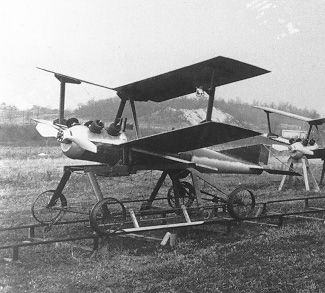
\includegraphics[width=0.5\textwidth]{kettering_bug.jpg}
    \caption{The Kettering Bug (1918)}
    \label{fig:ketteringbug}
\end{figure}

Throughout the 20th century, UAVs become more and more sophisticated, and were used more and more, but always for military purposes. In the more recent years, civilian UAVs have started to appear on the markets and their number quickly exceeded that of military UAVs. In February 2017, the FAA (Federal Aviation Administration) of the United States estimated that around 1.1 million units were in use in the US alone, and expected that number to rise to 3.55 million by 2021 \cite{consumerdronesbythenumbers}. These civilian drones are very different from military drones, in both their form and their function: civilian drones are usually smaller, and use rotors to take off vertically. They are used in a wide variety of applications.

\section{Motivation}
The ability to remote-control small and agile flying objects over large distances through the air, and to bring them to previously inaccessible locations, makes many new things possible. With the increasingly lower prices and better performances of civilian UAVs, people keep finding more and more uses for these high-tech gadgets. Some examples of these applications are: crop monitoring in agriculture \cite{agriculturaldrones}, delivery of mail or parcels, construction \cite{batiravecdesdrones}, cinematography, entertainment, or search and rescue operations. In all these applications, the more autonomous a drone is, the more efficient it will be at its task. One of the main challenges to achieve autonomy is for an UAV to be able to correctly identify its surroundings, and localize itself within them. In outdoor environments, GPS systems allow UAVs to know their position with great accuracy, but this is not possible in GPS-denied environments, like inside buildings. The main subject of this thesis will be fully autonomous navigation by a quadcopter in a GPS-denied environment.

\subsection{Ethical considerations}
The new possibilities brought by drones also pose ethical questions about security and privacy. Even though this technology can improve people's quality of life, it also has the potential to diminish it. If drones start to be widely used commercially, we could reach a point where the sound nuisances that they cause seriously impacts people who live in densely populated areas. Moreover, they can make us feel less at home, knowing that we could be observed from the sky at any moment. For this reason, it is important to adopt strict regulations regarding the use of drones in public spaces. Fortunately, many countries are already adopting legislation in this direction.


\section{Context}
This thesis is part of a project at the UCL that spans over several years and several masters theses. This project was launched by professor Julien Hendrickx in the 2012-2013 academic year, and had as long-term goal to develop a program that would enable low-cost UAVs to navigate autonomously in indoor environments. This means creating a map of their environment, localizing themselves in this map, and avoiding obstacles during exploration, using only on-board sensors. Another goal is to allow several drones to collaborate to speed up exploration. Five masters theses have already been written on this subject, each taking the work of the previous a little further.
\paragraph{2012-2015: First three theses}
In each of the three academic years (2012-2013, 2013-2014, 2014-2015), a masters thesis on the subject of indoor navigation for autonomous low-cost drones was written. These masters theses formed the base of the future work. They implemented visual SLAM methods to allow drones to build a two-dimensional map based on keypoints (first red pucks, then visual landmarks that the drone detected from a textured scene), and to localize itself within this map. During this time, inter-drone communication was also established, and was used to allow a drone to communicate the location of a target to another drone.

\paragraph{2015-2016: Recent work}
Last year, two groups of students simultaneously wrote theses on this subject. Before doing so, they joined forces to re-implement what had been done previously, but using ROS, a toolkit to develop software for robots that would make many things simpler, and allow more flexibility (see section \ref{sssec:ROS}).
The work of the first group of students allowed a drone to search and follow a mobile target, and call a second drone to continue this task when its battery was low.\\
The second group of students extended the SLAM algorithm to allow to use a 3D map to localize the drone. Unfortunately, they did not implement triangulation, so instead of projecting points into 3D space, they made the assumption that all points were located on the ground when building the map. The end result was a drone capable of using a 3D map to localize itself, but unable to build one from its observations.


\section{Objectives}
For this thesis, the goal is to continue the work of last year's second group to allow true 3-D SLAM: to build a 3D map based on observations by the monocular camera. To achieve this goal we will first follow these intermediate objectives:
\begin{itemize}
\item Research the current state of the art for 3D keyframe-based monocular visual SLAM
\item Implement a way to triangulate points based on multiple observations
\item Implement a way to use new visual information to correct previous errors and build a consistent map
\end{itemize}


\section{Ressources}

\subsection{Hardware}
For the practical implementation of this project, a Parrot AR.Drone 2.0 was used. This quadrotor was commercialized in 2012 and is an updated version of the original AR.Drone that was launched in 2010. This drone was marketed as a high tech toy, and is designed to be controlled from a smartphone application (connected to the drone via Wi-Fi). A few augmented reality games are available for the AR.Drone, in which it can visually recognize some predefined tags using its cameras, and interact with objects or other drones with a tag. To encourage the creation of more games for their drones, Parrot has released an open SDK that allows to effectively reprogram the drones. This early release of an open SDK has made it quite popular in the scientific community to do research on autonomous flight. The drone consists of 4 rotors, each with their own electric motor and microcontroller, an internal computer with a 1GHz ARM Cortex A8 processor and 1GB DDR2 RAM at 200MHz, and various sensors.

\subsubsection{Sensors}
The AR.drone has the following sensors:
\begin{itemize}
  \item 3 axis accelerometer with $\pm$  \SI{50}{\milli\gram} accuracy
  \item 3 axis gyroscope with $\pm$ \SI{2000}{\degree\per\second} accuracy
  \item Pressure sensor with $\pm$ \SI{10}{\pascal} accuracy
  \item 3 axis magnetometer with $\pm$ \SI{6}{\degree} accuracy
  \item Ultrasound sensor (facing downwards)
  \item Front camera (HD 720p 30 fps)
  \item Bottom camera (QVGA, 60 fps)
\end{itemize}

The accelerometer and gyroscope form the IMU, or Inertial Measurement Unit. During normal (remote-controlled) operation, the IMU is used to measure the speed of the drone, and stabilize it. The pressure sensor has a precision of \SI{10}{\pascal}, which is equivalent to about \SI{83}{\centi\metre}, so it is not precise enough to be a useful sensor indoors. Instead, the ultrasound sensor gives a very precise measure of the altitude of the drone. The magnetometer is used along with the IMU to estimate the drone's orientations. The bottom camera is used to estimate the drone's speed, by using optical flow methods. Finally, the front camera is not used for navigation, but for the user to see through the drone, and make films or take pictures. In this work, however, we will use the front camera as the main sensor of our Simultaneous Localization and Mapping algorithm, to detect and map visual features. In indoor environments, the front camera is the drone's sensor that has the potential to capture the most information about its surroundings. Unfortunately, this information comes in the form of images, and deducing useable information from these images is not a trivial task. The main focus of this work is to transform these images into useable information.


\subsection{Software}

\subsubsection{Closed-source internal code}
The code that runs on the drone during normal execution is unfortunately closed-source. This code receives a velocity command from the user via a smartphone app, and drives the drone according to this input. When no input is given, the drone stays stationary, in "hover mode". To achieve this, it fuses sensor information from the IMU, the ultrasound, pressure sensor, magnetometer, as well as odometry from the visual flow of the bottom camera to estimate its displacement, and uses this fused pose estimate to stabilize itself.

\subsubsection{Parrot SDK}
The software development kit released by Parrot allows to send commands and receive information from the drone. It is possible to send the drone commands to take off, land, emergency stop, hover, or move in a certain direction, but not to directly control the command send to the motors, or to have access at the control law used for the hover mode. Similarly, it is possible to read the IMU, ultrasound, odometry and video data from the drone, but not to access the data fusion that it does internally.

\subsubsection{ROS}
\label{sssec:ROS}
For the practical programming of the drone, this project uses the ROS (robot operating system) toolbox since last year. This toolbox provides useful abstraction to program robots: the program is decomposed into "nodes", each node running simultaneously in a separate thread. Each node implements part of the drone's task, and the nodes can communicate between each other by sending structured messages. The objective is to make the code modular, to be able to use existing nodes uploaded by other developers as part of packages. One such package, called "ardrone autonomy" developed by the Autonomy Lab of Simon Fraser University handles communication with a physical AR.Drone, so by using this node, we can completely disregard Parrot's specific SDK, and send all commands in ROS format. This way, we hope to make it easy to reuse code in case of a change of hardware. ROS also provides a number of convenient tools for developing software to be used on robots: it provides ways to record and replay data, to easily set and change parameters, and to cherry pick which parts of the program to run when doing tests.

\subsubsection{OpenCV}
OpenCV is an open-source computer vision library. It provides functions and data structures to manipulate images, and implements many state-of-the-art computer vision algorithms. It can work with ROS messages. We will use this library for all of our computer vision implementation: keypoint detection, tracking, description, and matching.

\subsubsection{PCL}
PCL stands for Point Cloud Library and is also an open-source library for 3D point cloud processing. The map created by the drone is a point cloud, and is saved as a PCL data structure. Currently, PCL is only used to visualize this map, but in the future, it can be used for higher-level functions like combining maps created by multiple robots, or reconstructing a dense representation of the map from a point cloud.

\subsubsection{Ceres Solver}
Ceres solver \cite{ceres-solver} is an open-source library for modeling and solving non-linear least squares problems. It is developed and maintained by Google, where it is used among other applications to estimate the pose of the Google street cars. Google released it to the public as open-source software in 2012 \cite{introducingceres}. It will be used in this thesis to solve Bundle Adjustment problems (see section ).%%TODO


\section{Outline}
First, the state of the art of miniature UAVs, computer vision, and simultaneous localization and mapping will be explored in chapter 2. Chapters 3 through 5 will present the main subject of this work: computer vision (Chapter 3), localization (Chapter 4), mapping (Chapter 5). The results will then be presented in chapters 6: simultaneous localization and mapping. Finally, chapter 7 will expose the main conclusions of this thesis, and describe the main challenges for further work.


%\chapter{State of the art}
%%% State of the art (chpt2)
\section{Drones}
When talking about autonomous drone navigation, it is important to be aware of what the current hardware is capable of doing, and how we can expect it to evolve in the near future. There is quite a large choice of civilian drones available to choose from on the market. Here, we will look at the main differences between the available choices.

\subsection{Number of rotors}
Multirotors, or multicopters, are defined as rotorcrafts with three or more rotors. Having more rotors enables them to maneuver in 3D space with fixed-pitch rotors, unlike helicopters, which have articulations at the bases of their rotors. The most common multirotors have 3, 4, 6, or 8 rotors, and are respectively called tricopters, quadcopters (or quadrotors), hexacopters, and octocopters. Having more rotors has the advantage of giving more agility, at the cost of more energy consumption, and therefore a shorter battery life. A free solid object in 3D space, such as a multicopter, has 6 degrees of freedom: 3 for translation and 3 for rotation. To be able to directly control each of these 6 degrees of freedom, it must be possible to give 6 independent controls to the drone. This means that tricopters and quadcopters are always under-actuated: they can't directly control all 6 degrees of freedom.
For example, quadrotors whose rotors are all in the same plane (as is almost always the case), can directly control all three of their rotational degrees of freedom, but only one translational degree of freedom, as they can only accelerate in the direction parallel to the rotation of their rotors. Therefore, to control their position in the plane perpendicular to the direction of gravity, they have to first adapt their roll and pitch, so that the resulting force of gravity and the thrust of their rotors points inside that plane. Most hexacopters also work this way, as their rotors are also often in the same plane. Some hexrotors, however, have tilted rotors, and are fully actuated  \cite{dexteroushexrotor}. \\
Octocopters on the other hand, are always over-actuated. One example, the Omnicopter, developed at ETH Zurich \cite{omnidirectionalav} can perform a \SI{360}{\degree} rotation along any axis, and move in a straight line in any direction, which enables it to perform complex and precise maneuvers. It is able to catch thrown ping-pong balls with a little net.

\section{Computer Vision}
\subsection{Keypoint Detection, Description, and Matching} \label{sec:sota_keypoints}
Keypoint detection will be at the basis of our work, as we will build a map to localize the drone, and this map will be made up of landmarks, visual features observed with the camera of the drone. Good keypoints need to be recognizable from a wide variety of viewpoints, and ideally be invariant to changes of illumination, scale, rotation, or occlusion. Here is a quick overview of some of the most important keypoint detectors and descriptors that exist in the literature.\\

\paragraph{Scale-Invariant Feature Transform (SIFT)} Published in 1999 by David Lowe from Columbia Univeristy, SIFT \cite{sift} is the reference in keypoint description, because it is quite robust. It uses the maxima and minima of a difference of Gaussian function of the image, rescaled at different levels. The image is blurred by Gaussian filters at different scales, and the difference between blurred images is taken. The result is an image without its highest spacial frequencies (noise) and lowest spacial frequencies (untextured parts of the image), leaving only a certain range of frequencies, that correspond to specific detail levels. The maxima and minima of the resulting image are considered to be corners, and become keypoints. Each keypoint is then described by a vector of size \num{128}, representing histograms of orientation in the pixels around the keypoint. SIFT keypoints are very robust to changes of viewpoint, occlusion and illumination. Their main drawback is the computational cost to find them and to extract their descriptor.

\paragraph{Speeded Up Robust Features (SURF)} %cite bay_surf
Inspired by SIFT and first published in 2006, Speeded-Up Robust Features \cite{surf} was a new kind of keypoint detector and descriptor. SURF uses square shaped filters to approximate Gaussian smoothing, which can be computed much faster, and then selects points where the determinant of the Hessian matrix is maximal. Its performance in terms of robustness to changes in viewpoint, occlusion, and illumination is similar to that of SIFT but it is computationally much faster.

\paragraph{Features from Accelerated Segment Test (FAST)}
Published in 2005, the FAST detector \cite{fast} uses a different approach than SIFT and SURF, and is even faster than SURF. FAST compares the intensity of a central pixel with the intensities of the 16 pixels forming a Bresenham circle of radius 3 around the central pixel. If the central pixel is brighter or darker by a certain threshold than N contiguous pixels in the circle, the pixel is considered a corner. This test is very fast, because it is possible to reject points that do not match the criteria without comparing the intensities of all points of the circle. The threshold and the number N are parameters that have to be fixed by the user. In the original version of FAST, $N = 12$ and the four pixels at the cardinal points of the circle (up, down, left, right) are first tested, and the point is rejected if the values of these four points make it impossible for N consecutive brighter or darker pixels to exist.
Expanding on this idea, the creators of FAST proposed an upgrade to their algorithm in \cite{fast2} using machine learning. Their upgrade uses the ID3 algorithm to learn a decision tree to decide whether a point is a keypoint or not using the intensities of the 16 pixels. This algorithm automatically selects to best tests to perform on these 16 pixels to quickly decide whether they are corners or not.
With this detector, the natural descriptor to use are the intensities of the 16 surrounding pixels, as well as whether the keypoint is a minimum or a maximum. We can already see that the dimension of the descriptor vector of FAST is 16, where SIFT's descriptor is of dimension 128, so we can expect this descriptor to be much less robust than SIFT.

\paragraph{Binary Robust Independent Elementary Features (BRIEF)}
BRIEF \cite{brief} is a descriptor introduced in 2010 that represents keypoints with binary strings. Each bit in the string is the result of a test testing which one of two specific pixels in the neighborhood of the keypoint is brightest in the smoothed image. Different lengths can be used for the string, but the creators of this descriptor found that a size of only 256 or even 128 bits is often enough for accurate matching. Matching between BRIEF features is done using the Hamming distance, which can be computed very quickly on modern computers.

\paragraph{Oriented FAST and Rotated BRIEF (ORB)}
In 2011 Rublee et al. \cite{orb} proposed a combination of a modified FAST detector, and a modified BRIEF descriptor, to obtain the ORB detector and descriptor. One of the main drawbacks of FAST is that is has no orientation component, so it is unable to recognize keypoints when these are rotated in the camera plane. ORB computes an orientation component to each keypoint detected by FAST by using the intensity centroid of the patch, and then computes a rotated BRIEF descriptor, so that the resulting keypoint is invariant to rotations. Because the FAST detector and BRIEF descriptor are both very fast methods, and result in very small descriptors, ORB keypoints are very efficient computationally.

\subsection{Bundle Adjustment}

\section{Simultaneous Localization And Mapping}
Simultaneous Localization and Mapping (SLAM) refers to the joint task of creating a map of a robot's surroundings, while also keeping track of the robot's location in this map. The word "robot" should be understood very broadly in this context, for example it could be a simple hand-held camera. Because there are countless different types of robots that do SLAM, SLAM is also a very diverse field, with different algorithms for different kinds of sensors.

\subsection{Parallel Tracking and Mapping (PTAM)}
PTAM \cite{ptam} was one of the first applications of Bundle Adjustment in real time. It is able to track the movement of a hand-held camera by constructing a map of visual features (it uses FAST). It is called parallel tracking and mapping, because the tracking and mapping tasks are completely decoupled, and happen simultaneously in different threads. However, it is quite expensive computationally, so it only works in real time with small workspaces, and lacks loop closure (the ability to correct accumulated errors when revisiting a previously visited location). PTAM has been adapted to work with Parrot AR.Drones at the Technische Universtät München \cite{engel2011msc} with impressive results, however this solutions suffers from PTAM's problems: the size of the map is quite limited, and there is no loop closure. As a result, the implementation if \cite{engel2011msc} builds an initial map, and then stops mapping, only using this initial map for tracking, which makes it unusable for large environments.

\subsection{ORB-SLAM}
ORB-SLAM \cite{orbslam}, created in 2015 is a keyframe-based monocular visual SLAM that builds a map of ORB features. The creators of ORB-SLAM extended it to ORB-SLAM 2 \cite{orbslam2}, which works with stereo and RGB-D cameras for better accuracy. It uses bundle adjustment to build a consistent map and for loop closure, and works in real time in large environments, by using a covisibility graph to focus the mapping and localization tasks on a small portion of the map at a time. It also uses a survival of the fittest approach to remove redundant keyframes and points.

\subsection{Large-Scale Direct Monocular SLAM (LSD-SLAM)}
Developped at the Technishe Universität München in 2014, LSD-SLAM \cite{lsdslam} uses a semi-dense approach to SLAM. Unlike the previously mentioned methods, it does not use keypoints, but rather, the entire image. Each new image is used to estimate a similarity transform from the previous image to estimate the position of the camera, and is then used to either refine the last keyframe, or create a new one. Each keyframe consists of an image and a depth map created with per-pixel stereo comparisons between consecutive images. The result works in real time on a CPU, and is able to obtain accurate maps of large environments, and to correct accumulated errors after loop closure.

\subsection{Direct Sparse Odometry (DSO)}
Also produced at the TUM, DSO \cite{dso} was created in 2016. Like LSD-SLAM, DSO is a direct method: it works directly on the image pixels by computing an associated depth field, instead of extracting keypoints from the image. Working directly on the image allows to bypass the costly point detection and description steps, and also allows to use points that are not recognizable by themselves, making more data useable (edges, weak intensity regions) and to work in less textured environments. Unlike LSD-SLAM, DSO is a sparse method, it samples a limited number of points on each keyframe, and does not use a smoothness geometry prior. Because DSO permanently marginalizes old points, it cannot detect a loop closure and correct accumulated errors, so it is more a pure visual odometry than a complete SLAM system, and cannot be used to obtain a consistent map (if it visits the same location twice, all points will be doubled). However, it is very accurate, and even after very large loops, the accumulated error remains small. Figure \ref{fig:dsodrift} shows an illustration of the accumulated error of DSO after going through an entire subway station.

\begin{figure}[H]
  \centering
  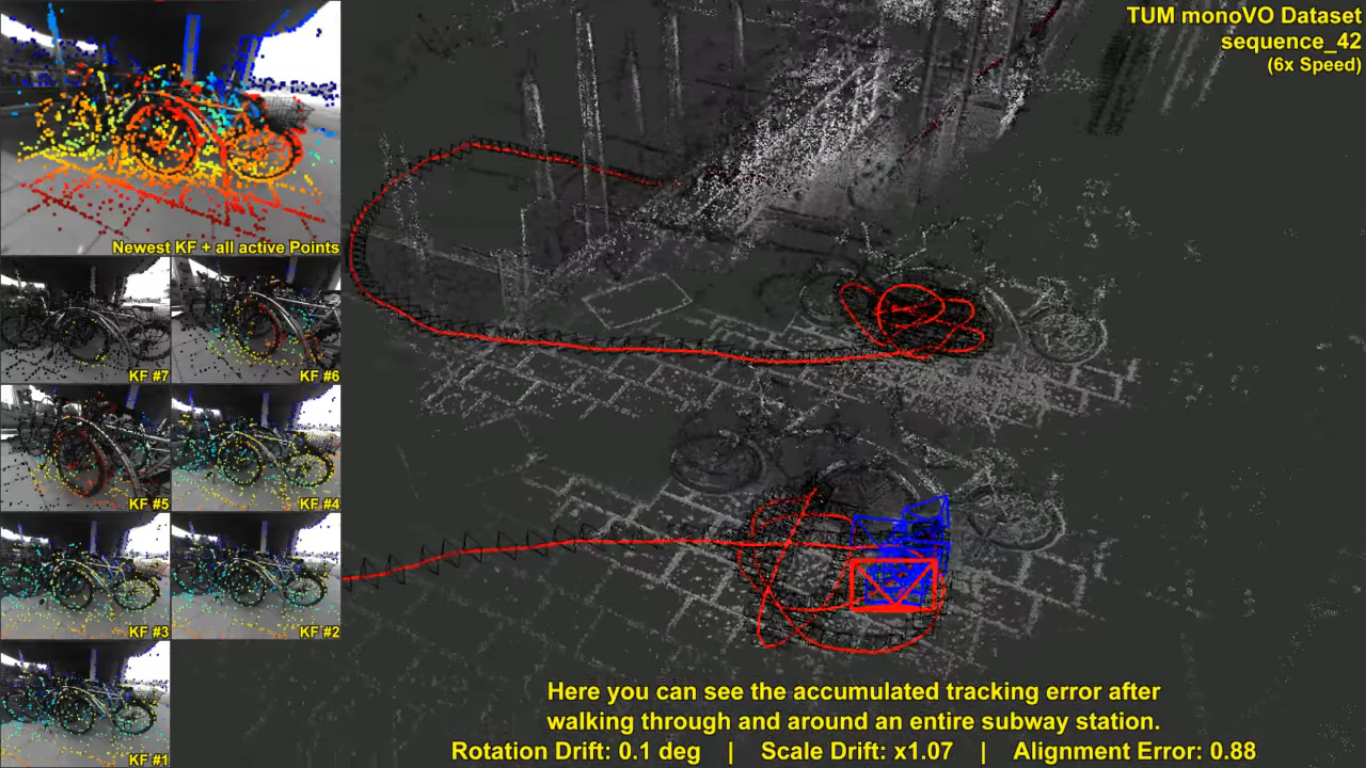
\includegraphics[width=0.5\textwidth]{dso_drift.png}
    \caption{Drift of DSO after going through an entire subway station. \cite{dsovid}}
    \label{fig:dsodrift}
\end{figure}

\subsection{SVO}

\subsection{CNN-SLAM}


%\chapter{Hardware and software architecture}
%%%Hardware and software architecture (chpt3)
\section{Hardware}
For this project I used Parrot's AR.Drone 2.0. This quadrotor was commercialized in 2012 and is an updated version of the original AR.Drone that was launched in 2010. This drone was marketed as a high tech toy, and is designed to be controlled from a smarphone application (connected to the drone via Wi-Fi). A few augmented reality games are available for the AR.Drone, in which it can recognise some predefined tags using computer vision, and interact with abject or other drones with a tag. To encourage the creation of more games for their drones, Parrot has released an open SDK that allows to effectively reprogram the drones. This early release of an open SDK has made it quite popular in the scientific community to do research on autonomous flight. The drone consists of 4 rotors, each with their own electric motor and microcontroller, an internal computer with a 1GHz ARM Cortex A8 processor and 1GB DDR2 RAM at 200MHz, and various sensors.

\subsection{Sensors}
Tha AR.drone has the following sensors:
\begin{itemize}
  \item 3 axis accelerometer with $\pm 50$ mg accuracy
  \item 3 axis gyroscope with $\pm 2000\degree/s$ accuracy
  \item Pressure sensor with $\pm 10 \texttt{Pa}$ accuracy
  \item 3 axis magnetometer with $\pm 6\degree$ accuracy
  \item Ultrasound sensor (facing downwards)
  \item Frontal camera (HD 720p 30fps)
  \item Ventral camera (QVGA, 60 fps)
\end{itemize}


\section{Software}

\subsection{Parrot SDK}
The SDK released by Parrot allows to send commands and receive information from the drone. However, it does not allow acces to the lowest-level parts of the drone. It is possible to send the drone commands to take off, land, emergency stop, hover, move in a certain direction, but not to directly control the command send to the motors. Similarly,


\subsection{ROS}


%\chapter{Localization}
%%%Localization (chpt4)


\chapter{Mapping}
%% Mapping (chpt5)
\chapter{Mapping} %10
The task of mapping was the main challenge of this work. This task consists in determining the 3D coordinates of recognizable features, that can later be used as landmarks by the drone to estimate its own position. The main challenge when building a 3D map using a single monocular camera, is that a point needs to be observed from at least 2 different positions to be mapped. The simplest approach to map a point, is to simply triangulate its position from two different views. We will begin by exploring this approach. We will find that although this does work reasonably well when we are certain of the position of the cameras, it does not when this position is uncertain. In addition, this method does not allow to take more than two observations of any point into account.\\

To remedy these problems we will implement a bundle adjustment step, that allows to build a map that is globally consistent. Throughout this section, we will have to make design choices to try to obtain a method that is both fast enough to work in real time, and accurate enough for the drone to control its position.\\

Finally we will implement a mapping strategy, that decides when and how to grow or reduce the map, and how to initialize it.

\section{Structure of the map}
We will keep the keyframe-based structure for the map from the previous years, but this structure will need to be adapted so that each landmark does not belong to just one keyframe. The map will contain two main data structures: a list of keyframes, and a list of landmarks. Each keyframe will contain the following information: the drone's pose estimation at the moment the keyframe was created, the estimated corrected pose of the keyframe, a list of observed keypoints. For each observed keypoint of this list, we also save its descriptor, its 2D position in the image plane of the keyframe, and whether it corresponds to a landmark of the map, and which one. Each landmark will contain a descriptor, its estimated 3D coordinates, and a list of keyframes seeing it. The map can be seen as a bipartite graph, where the landmarks and the keyframes form the two sets of nodes, and where an edge is present between a landmark and a keyframe if the keyframe sees the landmark.\\

The map grows every time we decide to add a keyframe. When we do, the keypoints of the current image seen by the camera, along with their 2D coordinates and descriptors, are saved in a new keyframe. The descriptors are then matched with descriptors of the other keyframes, and when there is a match between two keypoints of two different keyframes, we can triangulate a new landmark into the map.\\

\section{Triangulation} \label{sec:triangulation}
Our first problem is where to put a landmark in the 3D world from two observations at two different keyframes. If all measurements were perfect, we could simply draw a ray at each keyframe that goes from the camera center and passes through the keypoint in the image plane, and those two rays would intersect at the position of the landmark. \\

Unfortunately, those lines never intersect in practice, due to various errors (measurement errors, errors in the model of the cameras, errors on the position estimation of the cameras), so we need to find a method to locate a 3D point as best as possible from the pair of images.

\begin{figure}[H]
\centering
\begin{subfigure}{.5\textwidth}
  \centering
  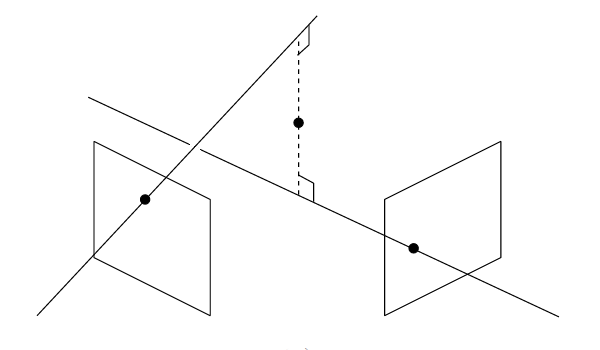
\includegraphics[width=\linewidth]{triang_midpoint.png}
  \caption{Midpoint method}
  \label{fig:midpoint}
\end{subfigure}%
\begin{subfigure}{.5\textwidth}
  \centering
  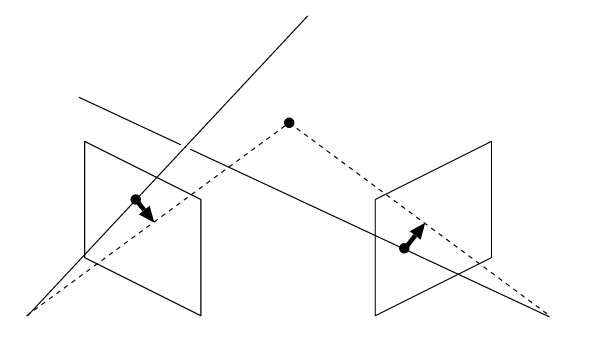
\includegraphics[width=\linewidth]{triang_optimal.png}
  \caption{Optimal Correction}
  \label{fig:optimalcorrection}
\end{subfigure}%

\caption{Triangulation methods}
\label{fig:triang}
\end{figure}

\subsection{Midpoint Method}
The simplest and most obvious solution is to take the midpoint of the common perpendicular of the two rays. This method is intuitive to understand geometrically, and is quite easy to compute. In practice, however its results are not very good, as there is no theoretical reason for this point to be the best.

\subsection{Optimal Correction}
If we assume that the error on observed points is random and follows a Gaussian distribution with zero mean, then the optimal solution would be to displace the pixels on both images until the resulting rays meet, keeping the displacement of the pixels as small as possible in the least squared sense. Such a solution would give the maximum likelihood estimator of the position of the 3D point, under those assumptions.\\

There are several algorithms in the literature that triangulate the position of a point using optimal correction. The most popular one, proposed by Hartley and Sturm \cite{hartleysturm}, computes the solution directly but requires finding the root of a 6th degree polynomial. Kanantani et. al.'s method \cite{kanatani} finds a solution iteratively, but requires very few iterations to have an accurate solution, and in practice, is faster than the Hartley Sturm method. It also has better numerical properties, as unlike the Hartley-Sturm method, it does not have singularities at the epipoles.\\

As we will see in the results section (\ref{sec:comparetriang}), optimal correction performs better than the midpoint method, as could be expected. The performance increase from optimal correction is not very big however, because the biggest source of error is not Gaussian noise on the measurements of the points, but errors in the position estimate of the cameras at the moment of creating the keyframes.

\subsection{Angle between the rays}
It is interesting (and will be useful) to note that the accuracy of the triangulation depends on the angle between the two rays reaching the point. In the most extreme case, one of the two points from which the landmark is seen is exactly between the landmark and the other point, like on figure \ref{fig:anglesa}. Then the rays are parallel, the angle between them is \SI{0}{\degree} and the distance to the landmarks can't be determined. The same applies if the landmark is between the two points of view, and the angle is \SI{180}{\degree}, like on figure \ref{fig:anglesb}. The optimal situation lies between these two extreme cases, when the two rays form an angle of \SI{90}{\degree} like on figure \ref{fig:anglesc}. In practice, however, our scene is sufficiently far away so that this angle is always lower than \SI{90}{\degree}, so the larger the angle, the better.
\begin{figure}[H]
\centering
\begin{subfigure}{.28\textwidth}
  \centering
  
\includegraphics[width=\linewidth]{anglesa.eps}
  \caption{}
  \label{fig:anglesa}
\end{subfigure}%
\begin{subfigure}{.28\textwidth}
  \centering
  
\includegraphics[width=\linewidth]{anglesb.eps}
  \caption{}
  \label{fig:anglesb}
\end{subfigure}%
\begin{subfigure}{.28\textwidth}
  \centering
  
\includegraphics[width=\linewidth]{anglesc.eps}
  \caption{}
  \label{fig:anglesc}
\end{subfigure}%
\caption{Effect of the angle between the rays}
\label{fig:angles}
\end{figure}

\section{Bundle Adjustment}\label{sec:bundleadjustment}
Having a bad estimation of the keyframe's pose is problematic, as it will result in badly located landmarks, which in turn will cause a bad estimation of the camera's position when future keyframes are created. In the long term, errors will accumulate, and the map will be completely distorted. Luckily, if we have enough point correspondences between two images, it is possible to deduce the relative displacement between the two images. This means that from a set of images, we can reconstruct a scene, without even needing a prior estimation of the position of the cameras that took the images. This is good news as it means that the images can give us some absolute information about the scene, that can be used to correct the errors on the camera poses of the previous keyframes.\\

The problem of adjusting camera poses and 3D point locations in order to minimize the reprojection errors of the 3D points onto the image planes is known as bundle adjustment. Because bundle adjustment uses new information to correct older parts of the map, it allows to reduce the accumulation of errors. Another advantage of bundle adjustment, is that it can easily take into account points that are seen by more than two cameras, which is not trivial for the triangulation techniques described above. The main disadvantage of bundle adjustment is that it is computationally heavy, so it is important to adapt it to make it useable in real time.\\

Bundle Adjustment an optimization problem of a nonlinear least-squares problem. The problem can be described as follows:

\subsection{Variables and constants}
We are simultaneously trying to determine the layout of the drone's surroundings (landmarks) and to correct the estimations of the drone's poses at the previous keyframe locations. The variables we are optimizing are the previous keyframe poses and the 3D locations of the landmarks. Let $\mathcal{K}$ be the set of keyframes, $\mathcal{L}$ be the set of landmarks and $\mathcal{L}_k$ be the set of landmarks observed by keyframe $k$. We will call the camera centers of the previous keyframes $\mathbf{c}_k$ and their roll-pitch-yaw orientation angles $\mathbf{r}_k$. The 3D position of the landmarks will be called $\mathbf{p}_l$. For each observation of a landmark by a keyframe, we know at what 2D point on he image that point was observed. Let $\mathbf{i}_{lk}$ be the image coordinates of landmark $l$ in keyframe $k$.

\begin{table}[H] \caption{Table of notation for Bundle Adjustment}
  \centering
  \begin{tabular}{r c p{10cm} }
  \toprule
  \multicolumn{3}{c}{}\\
  \multicolumn{3}{c}{\underline{Constants}}\\
  \multicolumn{3}{c}{}\\
  $\mathcal{K}$   & $\triangleq$ & Set of keyframes\\
  $\mathcal{L}$   & $\triangleq$ & Set of landmarks\\
  $\mathcal{L}_k$ & $\triangleq$ & Set of landmarks seen by keyframe $k$\\
  $\mathbf{i}_{lk}$        & $\triangleq$ & Image coordinates of landmark $l$ in keyframe $k$'s image plane\\
  \multicolumn{3}{c}{}\\
  \multicolumn{3}{c}{\underline{Decision Variables}}\\
  \multicolumn{3}{c}{}\\
  $\mathbf{c}_k$           & $\triangleq$ & Position of camera center of keyframe $k$\\
  $\mathbf{r}_k$           & $\triangleq$ & Roll-pitch-yaw angles of camera of keyframe $k$\\
  $\mathbf{p}_l$           & $\triangleq$ & Position of landmark $l$\\
  \bottomrule
  \end{tabular}
  \label{tab:banotation}
\end{table}

$\mathrm{Proj}(\mathbf{p},\mathbf{c},\mathbf{r})$ is the projection operator. it transforms the 3D point coordinates $\mathbf{p}$ of any point into the 2D image coordinates of that point if it were perfectly observed by a keyframe located at position $\mathbf{c}$ with orientation $\mathbf{r}$. In addition of depending on the extrinsic camera parameters, ($\mathbf{c}$, and $\mathbf{r}$), this operator depends on the intrinsic (focal length, projection center, skew) parameters of the camera. In general, bundle adjustment refers to the problem of adjusting both the intrinsic and extrinsic camera parameters of the different keyframes, but in our case, the same camera is used at every location, and the intrinsic parameters have been found in advance using camera calibration. Therefore, we can simplify our model by taking the intrinsic parameters as known constants, and only solving for the extrinsic parameters and the position of the landmarks.

\subsection{Objective function} \label{sec:loss}
We want to minimize the reprojection error of the observed landmarks. After estimating $\mathbf{p}_l$, the position of landmark $l$, we can re-project point $l$ into the images it was observed from. For example, $\mathrm{Proj}(\mathbf{p}_l,\mathbf{c}_k,\mathbf{r}_k)$ is the reprojection of point $l$ into the image plane of camera $k$. We can then compare the reprojection with the actual observation of point $l$ by camera $k$ to find out how consistent the estimation of the position of point $l$ is with the estimation of the position and orientation of keyframe $k$. The objective then becomes:
\begin{equation} \label{eq:objfunc}
  \min \sum_{k\in\mathcal{K}}\sum_{l\in\mathcal{L}_k} L(\mathrm{Proj}(\mathbf{p}_l,\mathbf{c}_k,\mathbf{r}_k) - \mathbf{i}_{lk})
\end{equation}
for some loss function $L(\cdot)$. We would like to use a squared loss function, as it has good computational properties, but it has the disadvantage of giving a lot of weight to outliers. If some landmarks result from bad point correspondences, their reprojection errors will be very large, so they will influence the end result quite a lot. To reduce the effect of outliers, we use a more robust loss function: the Huber loss function.
\begin{equation} \label{eq:huber}
  L_\delta(x) = \left\{ \begin{array}{l l}
    \frac{1}{2} x^2 & \mathrm{if } |x| \leq \delta \\
    \delta|x| - \frac{1}{2}\delta^2 & \mathrm{otherwise} \end{array} \right.
\end{equation}
This function is equal to squared loss for values of $x$ smaller than $\delta$, and becomes straight line elsewhere. \\

Note that if we kept the keyframe positions and orientations constant, and if there were only 2 keyframes observing each landmark, then the triangulation obtained with optimal correction would already give us the landmark positions that minimize this reprojection error. The interest of using bundle adjustment is that it allows to correct the positions of the camera at the keyframes, and to consider more than two observations per landmark.

\subsection{Constraints}
Bundle Adjustment is generally an unconstrained problem, but we will add some soft constraints to incorporate information we have from the sensors. We will add terms to the objective function that penalize keyframes whose altitude, roll, and pitch are far away from the ones measured during the keyframe creation. Because each of these measures is absolute, they are not subject to drift, so they should be accurate even after the drone travels large distances. Doing this will prevent the solution of the bundle adjustment taking unrealistic values. \\

Another advantage is that this will (softly) fix the scale. As we said before, monocular vision only gives information of the world up to a scale factor, and bundle adjustment is normally unable to recover the real scale of the map it builds. Enforcing a constraint on the altitude of the keyframes fixes this scale, on the condition that the altitudes of the different keyframes vary, because then it gives a constraint on the distance between keyframes. For this reason, making the second keyframe from a position directly above the first one is a good idea.


\subsection{Solver}
We have a least square problem of the form:
\begin{equation} \label{eq:solver}
  \min_{x} G(x) = ||F(x)||^2
\end{equation}
Where $F$ is a highly non-linear, non-convex function as defined in \ref{eq:objfunc}. Because F is non-linear and non-convex, we can only hope to minimize it locally, using an iterative algorithm, so it will be very important to start from initial solutions that are close to the optimum. At each iteration, we want to find a step $\Delta x$ that brings the objective $F(x+\Delta x)$ closer to zero. We use the first-order approximation of $F(x + \Delta x)\approx F(x) + J(x)\Delta x$, where $J(x) = \left[\frac{\partial F_i}{\partial x_j}\right]$ is the Jacobian of $F$. Deriving \ref{eq:solver} with respect to $\Delta x$ with this approximation and setting it to zero gives the Gauss-Newton update:
\begin{equation}\label{eq:gaussnewt}
	\left( J^TJ\right)\Delta x = -J^TF
\end{equation}
By adding a regularization term $\lambda I$ to equation \ref{eq:gaussnewt}, we obtain Levenberg's update:
\begin{equation}
	\left( J^TJ + \lambda I \right)\Delta x = -J^TF
\end{equation}
Marquardt later improved this update by replacing $\lambda I$ by $\lambda\texttt{diag}(J^TJ)$, for faster convergence when $\lambda$ is large.\\

When the value of $\lambda$ is very small, the Levenberg-Marquardt update is quite close to a Gauss-Newton update, and when it is large, it becomes close to a gradient update. The Levenberg-Marquardt algorithm can be seen as a hybrid between the two. After each iteration, $\lambda$ is increased if we are getting closer to a minimum, or decreased if the iteration results in a worse value of the objective function. As a result, when the $2^{nd}$ order approximation is good, the method is close to a Gauss-Newton method, and very fast, and when it is bad, the method reverts to a gradient descent for stability.\\

To measure how good the approximation is we use $\rho$, a metric to compare the gain in the objective function with the one we would have gotten if the approximation was exact:
\begin{equation}\label{eq:metric}
	\rho = \frac{G(x) - G(x + \Delta x)}{G(x) - ||(F(x) + J(x)\Delta x)||^2}
\end{equation}
After each iteration, if $\rho$ is above some threshold, we perform the step : $x_{\texttt{new}} =x + \Delta x$ and $\lambda$ is decreased by some factor, if not, we do not update the value of $x$, and $\lambda$ is increased. We stop the algorithm when either the gradient, or the relative update of the parameters ($|\frac{\Delta x}{x}$) falls below some threshold. \cite{levmar}


\section{Mapping Strategy}\label{sec:mapstrat}
The last remaining task of the mapping task is to put all these elements together to build the mapping algorithm. This algorithm needs to decide how to initialize the map, when to create new keyframes, when and how to run bundle adjustment, and how to limit the growth of the map.

\subsection{Map Initialization}
Because of the chicken-and-egg nature of SLAM (an estimate of the position is necessary to place landmarks, but a map is necessary to estimate the position), a special procedure is needed to initialize the map. Arbitrarily, we decide to place the origin of our reference frame at the pose of the drone where it creates the first keyframe, with the x direction pointing forwards, the y direction to the left, and the z direction upwards (this is the coordinate system used by \texttt{ardrone\_autonomy}). The first keyframe will serve as the anchor of the map: its position will never change, and will always stay at the origin.\\

A single keyframe is not enough to initialize a map, because two views of keypoints are required to triangulate them. This means we have to fly blindly to the location of the second keyframe before we can create any landmarks, and begin to estimate the drone's position using the map and PnP. The only available sensors during this first, blind flight are the IMU, the ultrasonic sensor, and the bottom camera (for optical flow). Of these, only the ultrasonic sensor gives an absolute measurement of position, the others all measure speed, and this speed estimation has to be integrated to give a displacement estimate. For this reason, we will mostly rely on the ultrasonic sensor to estimate the relative displacement between the two first keyframes. Because the ultrasonic sensor only gives the distance from the bottom of the drone to the ground, the drone should fly straight up from its first position (the origin) to reach its second position.\\

Once in its second position, the drone can match seen keypoints from both views, and from its estimated position, triangulate those points to the map. Then, using bundle adjustment, the error in the estimation of the displacement between the two first keyframes can be corrected.

\subsection{Local and global bundle adjustment}\label{sec:locglob}
As we will see in chapter \ref{chpt:results}, the time taken for bundle adjustment will be one of the major obstacles of this work. This time taken depends on the number of points and keyframes concerned, so as the map grows, it will become impractical to run bundle adjustment on all of it. For this reason, we will only solve bundle adjustment on a subset of the map, considering only the most recent keyframes, and the points seen by them. This will allow to put a cap on the size of the problem that has to be solved each time a keyframe is created. Confining bundle adjustment to a local window means that errors will still accumulate over time, but still much more slowly than with no bundle adjustment. To solve this, we can occasionally run bundle adjustment on the whole map, which would be especially useful if the drone revisits a previously seen location.

\subsubsection{Local Bundle Adjustment}
Every time a keyframe is created, we follow this creation with a round of local bundle adjustment, to correct the error due to the inaccuracy of this keyframe's position. When running local bundle adjustment, we only solve a sub-problem of the full bundle adjustment. In this sub-problem, we only consider the $n$ last keyframes, and the landmarks seen by at least two of those $n$ keyframes.\\

We will set the poses of the two oldest keyframes considered in the local bundle adjustment as constant. This is necessary to prevent drift. It there was no keyframe set as constant, the entire map could be shifted with no effect on the objective function. Likewise, if there was only one keyframe set as constant, the entire map could be scaled by a factor around the constant keyframe, with no change to the objective function. The two constant keyframes serve as anchor of the local map, fixing its position within the global map. Choosing the oldest keyframes to be set as constant ensures that the constant keyframes have already been through some ($n - 2$) rounds of local bundle adjustment, so we can expect their position to already be close to the correct one, or at least to be locally consistent with the map.

\subsubsection{Global Bundle Adjustment}
As local bundle adjustment only considers a sub-problem, its solution is not optimal with respect to the full problem. When the drone has processor time available, we can improve our solution by running the algorithm on the full problem. When doing this, we are modifying all keyframes except for the first one, the anchor of the global map. The keyframes that are normally kept constant during local bundle adjustment are also modified, correcting some of the accumulated error that was made until there. However, errors will still accumulate as the drone moves away from the global anchor. These accumulated errors can be corrected if there are loops in the drone's trajectory, but they do not prevent the drone from exploring because the map stays locally consistent.


\subsubsection{Loop Closure}
Each landmark couples the positions of all keyframes seeing them: modifying the position of one keyframe changes the optimal position of the landmark, which changes the optimal position of the other keyframes. We can consider keyframes to be neighbors if they see a common landmark. Having keyframes that are far away from each other, in the sense that many intermediate keyframes are required to go from one to the other, traveling from neighbor to neighbor, means that the two keyframes are very loosely coupled. The looser keyframes are coupled from the first keyframe, the more they are subject to drift, as the errors accumulate between them.\\

Using local bundle adjustment further increases this drift, as keyframes whose positions are not simultaneously optimized during bundle adjustment are only coupled through the anchors of the local bundle adjustment, not directly though point correspondences. When running global bundle adjustment, this drift can be corrected, especially when the keyframes are strongly coupled. The best situation for this is when the drone makes a full loop, and revisits locations seen by much older keyframes. The newest keyframes then become neighbors to the oldest, and global bundle adjustment can correct all the errors accumulated during the loop, resulting in a completely consistent map.

\subsection{Rejecting outliers}
When looking more closely at the results of bundle adjustment, we find that despite the use of a robust loss function (see section \ref{sec:loss}) a large part of the errors comes from a small number of points. Figure \ref{fig:errorrepartition} shows the repartition of contribution to the objective function between the landmarks (a logarithmic scale is used for the $x$-axis). We can see that \SI{1}{\percent} of the landmarks account for more than \SI{40}{\percent} of the total error, and that \SI{10}{\percent} of the landmarks account for more than \SI{80}{\percent} of the total error.  One possible explanation is that these points are bad matches, and do not correspond to real world points, so that even if we have the correct position of all cameras exactly, the rays corresponding to these points will not intersect.

\begin{figure}[H]
  \centering
  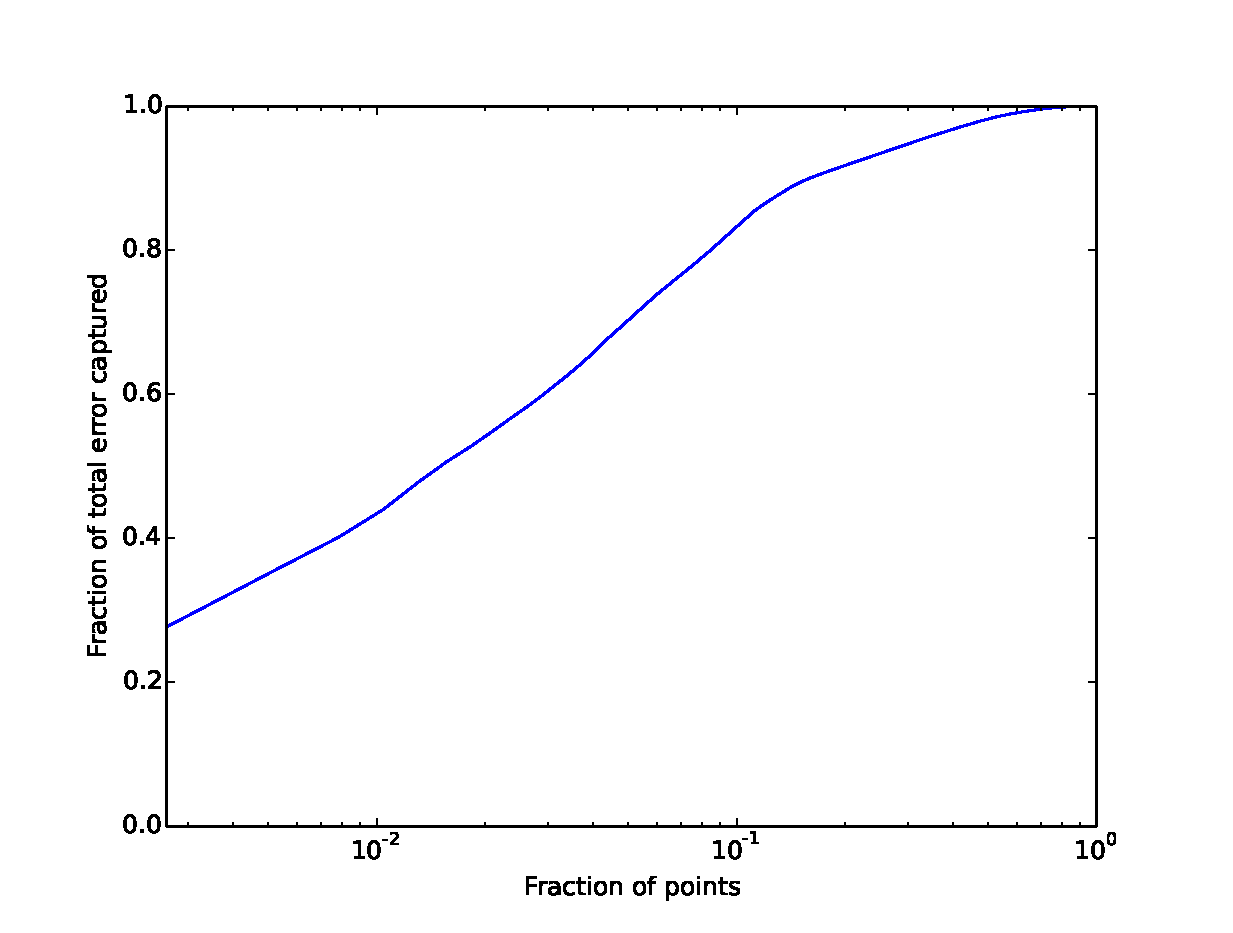
\includegraphics[scale=0.6]{err_repartition_4.eps}
  \caption{Repartition of error among points}
  \label{fig:errorrepartition}
\end{figure}

To solve this problem, after every bundle adjustment pass, we eliminate points whose error is higher than some threshold to be defined. Because the number of keyframes seeing each individual landmark varies, we should look at the error per observation of each point. It is also normal that the error per observation becomes larger for points observed by more keyframes, because every time an observation is added, the location of the point will change a bit, and its position will become less optimal with respect to the keyframes that already saw it.\\

For these reasons, we will put a different threshold on the points depending on the number of keyframes that see the point. If a point is seen by a large number of keyframes, we will allow it to have larger errors per observation before removing it.\\

As we will see in \ref{sec:outliers}, removing outliers greatly improves the performance.


\subsection{Choosing when to create keyframes}\label{sec:heuristic}
Choosing when to create keyframes was the most challenging task of this work. It is not a simple tradeoff between computation time and accuracy, as many (sometimes contradicting) points have to be kept in mind:
\begin{itemize}
\item Landmarks have to be observed from at least two keyframes before they can be used, so it is important to create keyframes sufficiently in advance
\item If two keyframes are too close to one another, the lines going from landmarks to these two keyframes will almost be parallel, causing a large uncertainty on the landmark's position
\item It is important to have a good pose estimate at the moment a keyframe is created, as this estimate will be the initial value of the keyframe's pose
\item Because when we add a keyframe we run a local bundle adjustment on the last $n$ keyframes, if the keyframes come in rapid succession, errors will accumulate faster, as there are more intermediates between the first and last keyframes.
\end{itemize}

The choice of when to create a new keyframe has to be made heuristically using any of the measures we have available. Amongst the quantities considered for this choice are:
\begin{itemize}
\item The time elapsed since the last keyframe was created
\item The distance to the position where the last keyframe was created
\item The distance to the position of other keyframes
\item The number of mapped points currently in the field of view
\item The number of unmapped points currently in the field of view
\item The number of inliers the last times RANSAC was run
\item Large areas in the field of view not containing any mapped points
\end{itemize}

After many trial-and-error tests, we came up with the following heuristic:

\begin{itemize}
\item{If bundle adjustment is currently running, don't create a keyframe}
\item{If the current position (disregarding orientation) is closer than \SI{10}{\centi\meter} to the last keyframe, don't create a new keyframe}
\item{The is no area larger than \SI{20}{\percent} of the image on any of the 4 sides that contains no RANSAC inliers}
\item{If any of the following conditions is true, create a new keyframe:}
\begin{itemize}
	\item{The current position (disregarding orientation) is farther than \SI{70}{\centi\meter} from the last keyframe}
	\item{An area larger than \SI{33}{\percent} of the image (from any of the 4 sides) contains no RANSAC inliers}
	\item{The current image contains less than 40 RANSAC inliers}
\end{itemize}
\end{itemize}

The reason we use the distance between poses, disregarding orientation, is that if one keyframe results from the drone performing a pure rotation from another keyframe, the rays between points of the scene and the keyframes will be close to parallel in the reference coordinate system, and cause resulting landmarks to have a large uncertainty. For this reason, it is also important that the path-planning node (not worked on in this thesis) avoids pure rotations.

\section{Summary}
Every time the mapping node receives a new frame from the computer vision node, it decides whether a new keyframe is needed, using the heuristic described in section \ref{sec:heuristic}. If a new keyframe is needed, the frame is transformed into a keyframe, the list of keypoints, each with their descriptor and 2D position on the image is saved, and the estimated position of the drone at the moment of creating the keyframe is assigned to the keyframe. The descriptors of the new keyframe are then matched with the descriptors of already mapped landmarks and with the descriptors of currently unmatched keypoints in older keyframes. If there is a match between two unmatched keypoints in different keyframes, a new landmark is created by triangulating its position with optimal correction (see section \ref{sec:triangulation}).\\

For each keypoint in each keyframe, we also save whether it corresponds to any landmark of the map. After the keyframe is created, we decide whether to run local or global bundle adjustment, as explained in section  \ref{sec:locglob}. We then run bundle adjustment (section \ref{sec:bundleadjustment}), either on the entire map if we decided to run global bundle adjustment, or on the last $n$ keyframes and the landmarks seen by at least two of those if we decided to run local bundle adjustment. Running bundle adjustment allows to use the matches between keypoints to correct the estimations of the positions of those keypoints and the keyframes seeing them.\\

Figure \ref{fig:mapflowchart} summarizes the mapping part of the code in the form of a flowchart. Bundle adjustment runs in a separate node, so that it doesn't block the entire mapping node.

\begin{figure}[H]
  \centering
  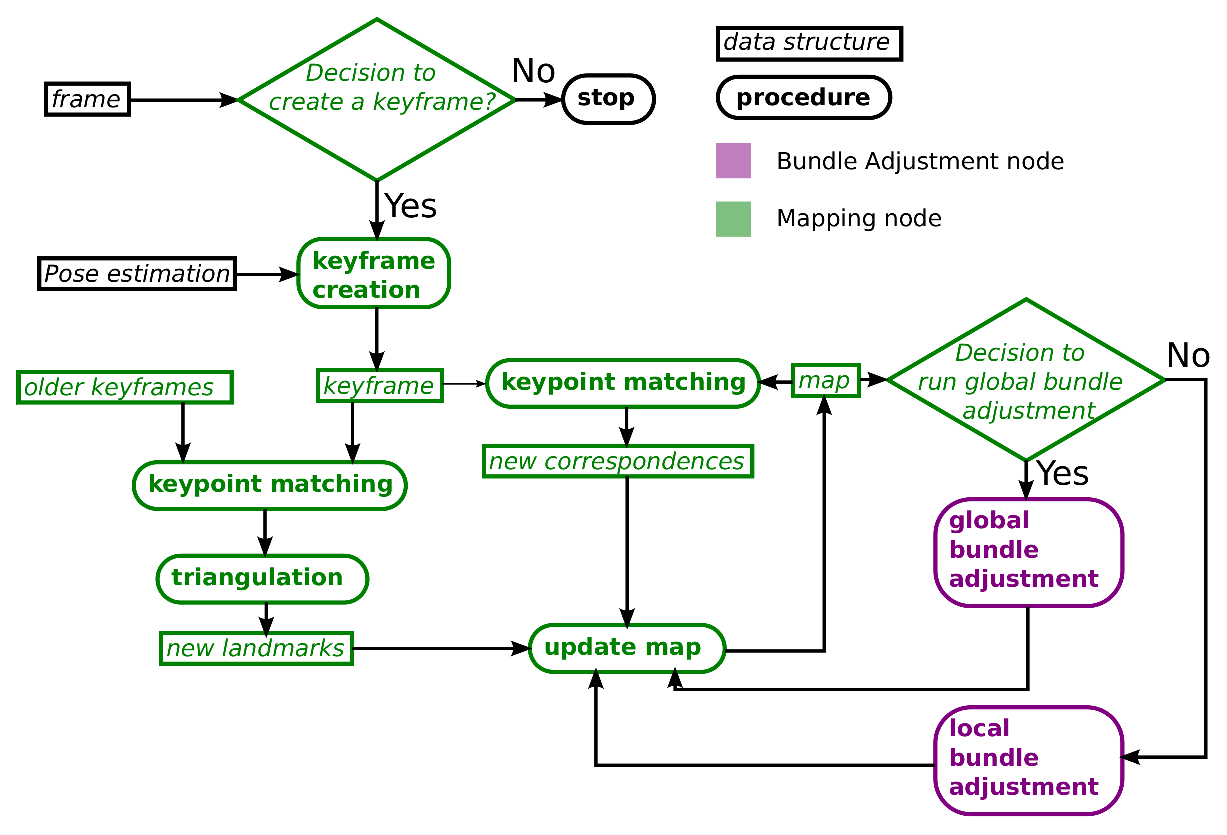
\includegraphics[scale=0.6]{mapflowchart.eps}
  \caption{Flowchart of the mapping task}
  \label{fig:mapflowchart}
\end{figure}


%\chapter{Simultaneous Localization and Mapping}
%%Simultaneous Localization and Mapping (chpt 07)


%\chapter{Conclusion}
%%%Conclusion (chpt6)


%\printbibliography%

\appendix
%\chapter{Benchmark results}
%\chapter{Full code flowchart}\label{app:flowchart}
\begin{figure}[H]
\centering
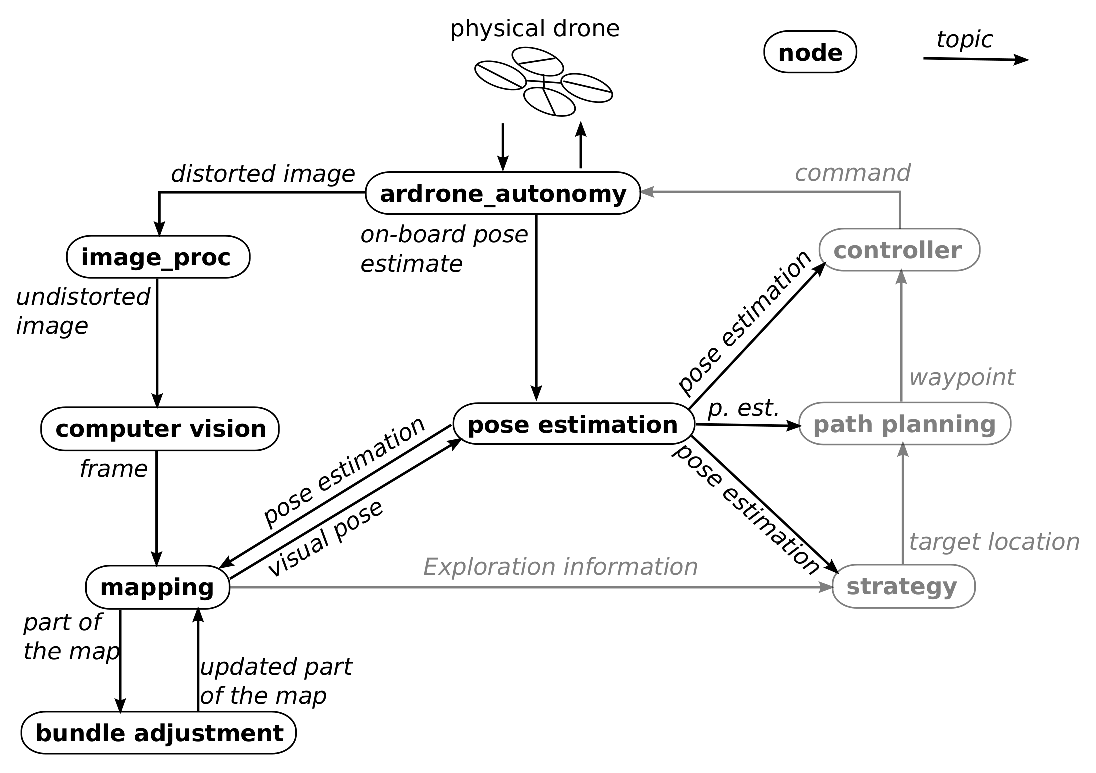
\includegraphics[width=\linewidth]{flowchart.eps}
\caption{Flowchart of the different nodes and the communication between them. Grayed-out parts were not worked on in this master's thesis}
\label{fig:fullflowchart}
\end{figure}


% Back cover page
\backcoverpage

\end{document}
